\documentclass[letter, 12pt]{article}
\usepackage[tmargin=1in,lmargin=1in,rmargin=1in,bmargin=1in,paper=letterpaper]{geometry}
\IfFileExists{minionpro.sty}
        {\usepackage[mathlf,textlf,minionint]{minionpro}}
        {\message{***Minion Pro not available***}}
% -------------------------------------------------------------
\usepackage{mathtools}
\usepackage{mathrsfs}
\usepackage{amsthm}
\usepackage{amsfonts}
\usepackage{framed}
\usepackage{enumerate}
\usepackage{ifthen}

\input{basicpreamble}
% -------------------------------------------------------------
\newif\ifpdf \ifx\pdfoutput\undefined
\pdffalse
\else
\pdftrue
\fi
\ifpdf
\usepackage[stretch=40,step=8,selected=true]{microtype}  % allow font expansion up to +/- 4% of normal width
\usepackage[pdftex]{graphicx}
\else
\usepackage[dvips]{graphicx}
\fi
% -------------------------------------------------------------
% END OF PACKAGES LOADED
\begin{document}

\parindent=0in
\newcounter{probnum}
\stepcounter{probnum}
\newenvironment{problem}[1][]
   {\begin{framed} \textbf{Problem \theprobnum: #1}}
   {\end{framed}\stepcounter{probnum}}
\newenvironment{bookproblem}[1]
   {\begin{framed} \textbf{Problem #1:}}
   {\end{framed}\stepcounter{probnum}}
%%%%%END OF HEADER

\begin{flushright}
Connie Okasaki \\
AMATH 584\\
Assignment 2\\
16 Oct 2020
\end{flushright}

\textbf{Yale Faces}

The code for this assignment can be found at https://github.com/cokasaki/amath584 ~\\

The $V$ matrix can be interpreted as a set of unit length, orthogonal "eigenfaces" which act as a basis for the training set. The $U$ matrix can be interpreted as being the decomposition of each actual face into loading coefficients for each eigenface. Finally, the $\Sigma$ matrix can be interpreted as measuring the relative importance of each "eigenface" in reconstructing the dataset: low singular values mean the eigenface has generally low coefficients across all faces. The singular value spectrum looks like the following (on a log-scale)
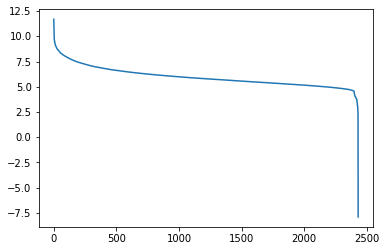
\includegraphics{logscale.png}
So the first 10-20 eigenfaces are by far the most important, and the last 100 or so are by far the least. We can see that the first 3 eigenfaces construct a generic average face
\begin{center}
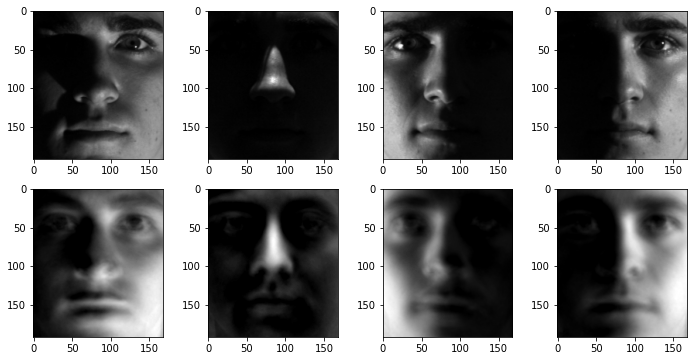
\includegraphics[width=0.8\textwidth]{reconstruction.png}
\end{center}
while the first 20 introduce major artifacts such as shadowing
\begin{center}
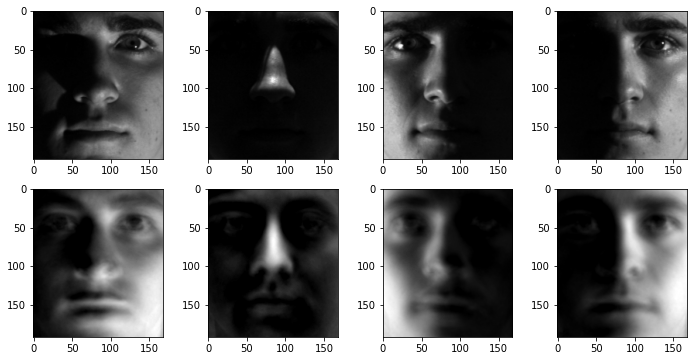
\includegraphics[width=0.8\textwidth]{reconstruction20.png}
\end{center}
Note that in order to construct these images we did have to bound the reconstructed vectors between 0 and 127. For the cropped faces, the eigenfaces provide useful insight into just what the basis vectors represent
\begin{center}
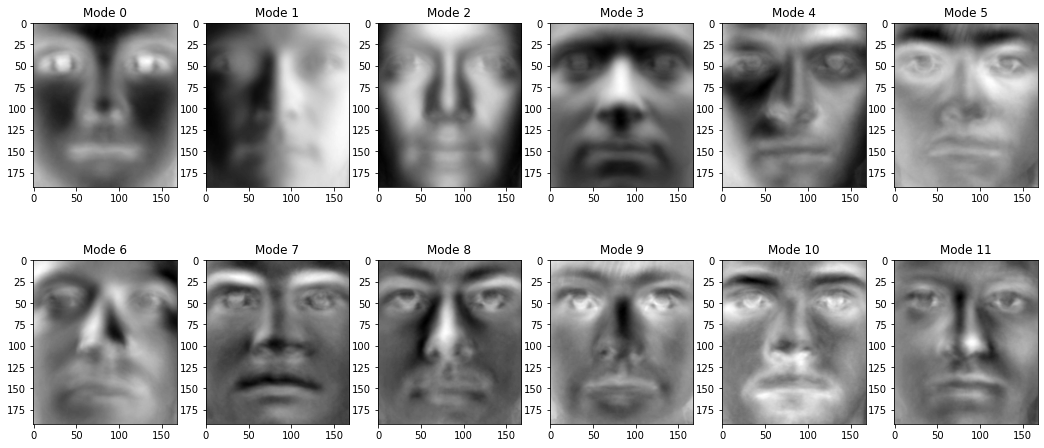
\includegraphics[width=0.8\textwidth]{modes.png}
\end{center}
We can see that for this dataset, most of the dominant modes represent actual interpretable facial features. In comparison, for the uncropped faces, the dominant modes largely represent positioning of the face in the image:
\begin{center}
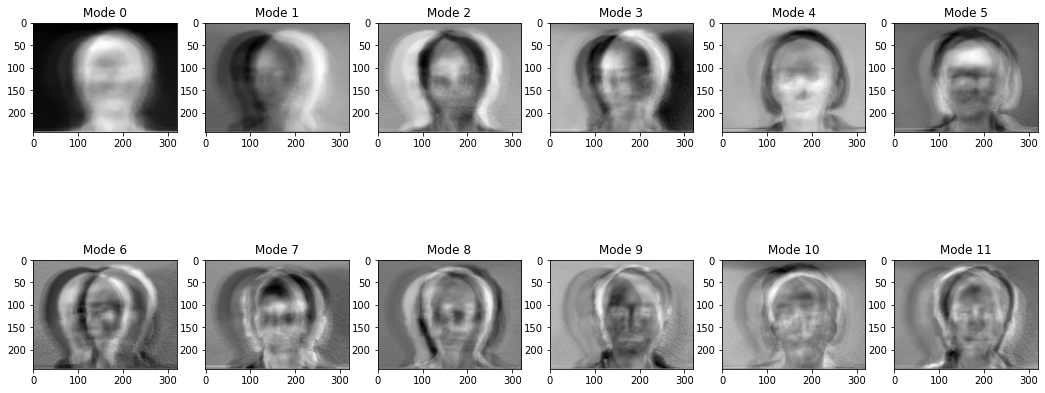
\includegraphics[width=0.8\textwidth]{position.png}
\end{center}
Due to this problem, image reconstruction is much poorer quality with even 20 modes providing only rough, blurred out features
\begin{center}
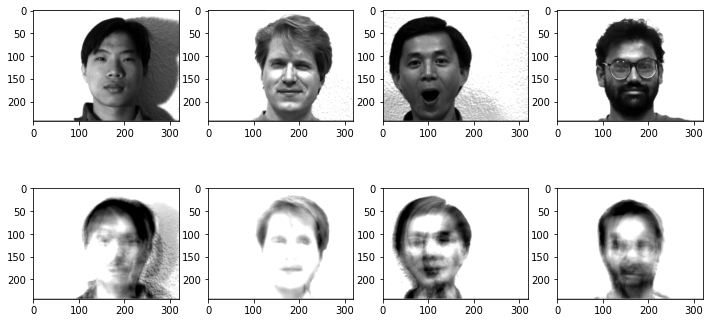
\includegraphics[width=0.8\textwidth]{uncropped_recon.png}
\end{center}
The decay, however, looks broadly similar:
\begin{center}
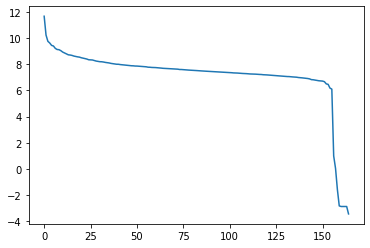
\includegraphics[width=0.8\textwidth]{uncrop_decay.png}
\end{center}

\pagebreak

%%=========== PROBLEM 1 ============= UNFINISHED ============%%
\begin{problem}
Show that for a matrix $A$
\begin{enumerate}[(a)]
\item The nonzero singular values of $A$ are the square roots of the nonzero eigenvalues of $AA^*$ or $A^*A$
\item If $A=A^*$, then the singular values are the absolute values of the eigenvalues of $A$
\item Given that the determinant of a matrix $U$ is unity, show $|\det(A)|=\prod_{j=1}^m \sigma_j$
\end{enumerate}
\end{problem}

\begin{enumerate}[(a)]
\item Suppose that the SVD of $A = U\Sigma V^*$, with singular values in descending order as usual. Then:
\begin{align*}
AA^* & = U\Sigma V^* V \Sigma^* U^* \\
& = U\Sigma\Sigma^* U^* \\
AA^* U = U \Sigma\Sigma^*.
\end{align*}
This is an eigenvalue problem. Since the singular values are real, we know that $\Sigma\Sigma^* = \Sigma^2$ so that the singular values are in fact the positive square roots of the eigenvalues of $AA^*$. Likewise
\begin{align*}
A^*A & = V\Sigma U^*U\Sigma V^* \\
& = V\Sigma^2V^* \\
A^*A V & = V\Sigma^2
\end{align*}
\item If $A=A^*$ then let $V$ be the eigenvalues of $A$. We know that $AV = V \Lambda$. But then $A^*AV = V \Lambda^2 = V\Sigma^2$. Thus, since the singular values are the positive square roots of $\lambda_i^2$ we see that they are the absolute values of the eigenvalues of $A$.
\item Presumably the problem is referencing the property that $|\det(U)| = 1$ for a unitary matrix. Therefore, \[|\det(A)| = |\det(U)|\times |\det(\Sigma)| \times |\det(V)| = |\det(\Sigma)| = \prod_{j=1}^m \sigma_j.\]
\end{enumerate}

\pagebreak

\end{document}